\documentclass[10pt, twoside]{article}
\usepackage[top=1in, left=1.5in, right=1.5in]{geometry}
\usepackage[parfill]{parskip}
\usepackage{fancyvrb}
\usepackage{amsmath}
\usepackage{mathtools}
\usepackage{hyperref}
\usepackage{multicol}
\usepackage{xcolor}
\usepackage{fancyvrb}
\usepackage{graphicx}
\graphicspath{{figs/}}
\usepackage{fancyhdr}
\IfFileExists{pdfx.sty}
  {
    \usepackage[a-1b]{pdfx}
  }{}
\newcommand{\secname}{}
\let\stdsection\section
\newcommand{\newsection}[1]{\clearpage\setcounter{numpar}{0}\stdsection{#1}\renewcommand{\secname}{#1}}
\newcommand\textgray[1]{\fcolorbox{gray!80}{gray!10}{\texttt{\bfseries#1}}}
\newcommand\texttb[1]{\texttt{\bfseries#1}}
\renewcommand{\section}{\clearpage\setcounter{numpar}{0}\stdsection}

\let\stdsubsection\subsection
\renewcommand\subsection{\setcounter{numpar}{0}\stdsubsection}
\let\stdsubsubsection\subsubsection
\renewcommand\subsubsection{\setcounter{numpar}{0}\stdsubsubsection}
\let\stdparagraph\paragraph
\renewcommand\paragraph{\setcounter{numpar}{0}\stdparagraph}
\newcommand\frelo{\relax}

\fancyhf{}
\fancyhead[LE,RO]{Dats language}
\fancyhead[RE,LO]{v2.0.0}
\fancyhead[CE,CO]{\bfseries DRAFT}
\fancyfoot[CE,CO]{\nouppercase{\secname}}
\fancyfoot[LE,RO]{\thepage}
\fancyfoot[RE,LO]{\frelo}
\pagenumbering{roman}
\renewcommand{\headrulewidth}{0pt}

\title{\textbf{The Dats\thanks{\url{github.com/dats-lang/dats-src/}} language v2.0.0}}
\author{"Dats dats dats da da dats dats dats"}
\newcounter{numpar}
\newcommand{\np}[1][]{%
  \par
  \refstepcounter{numpar}%
  \noindent
  \makebox[0pt][r]{%
    \makebox[0pt][l]{{\footnotesize\thenumpar}}%
    \qquad
  }%
  #1%
  \ignorespaces
}
\hypersetup{pdftitle={The Dats Language},
            pdfauthor={Al-buharie Amjari and others.},
            bookmarks=true,
            bookmarksnumbered=true,
            pdfpagelabels=true,
            pdfpagemode=UseOutlines,
            pdfstartview=FitH,
            linktocpage=true,
            colorlinks=true,
            linkcolor=blue,
            %plainpages=false
}

\pagestyle{fancy}
\setcounter{secnumdepth}{4}
\setcounter{tocdepth}{4}
\begin{document}
\maketitle
\thispagestyle{fancy}

\begin{Verbatim}[frame=single, label=The "Hello World" of Dats]
      staff foo {
        n 4, c4;
        n 4, d4;
        n 4, e4;
        n 4, f4;
        n 4, g4;
        n 4, a4;
        n 4, b4;
        n 4, c5;
      }

      main {
        track bar = synth.psg(foo);
        write("t.wav", bar);
      }
\end{Verbatim}
\begin{center}
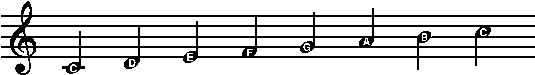
\includegraphics{notes/cdefgabc}
\end{center}

\vspace{0.5in}
\begin{abstract}
This is part of the Dats v2.0.0 documentation\footnote{\url{github.com/dats-lang/dats-tex/dats-2.tex}}
and is a draft. This document may be outdated in the future so readers are adviced instead to
follow 1, although this draft should be able to provide the syntax and able the user to
extrapolate from these to start writing a music composition in Dats language.


Recipients of this document are invited to give comments, suggestions and recommendations
for improvement of this current revision in a manner of constructive criticism.
Critics in this way are valuable and could help in formulating next appropriate
document.

Further revision of this draft may be publish by the author from time to time.
\end{abstract}

\clearpage
\vspace*{6in}

\begin{minipage}[t]{5in}
\begin{Verbatim}[fontsize=\small]
Copyright (c) 2021-2022 The Dats-TeX authors.

Permission is granted to copy, distribute and/or modify this
document under the terms of the GNU Free Documentation License,
Version 1.3 or any later version published by the Free Software
Foundation; with no Invariant Sections, no Front-Cover Text, and
no Back-Cover Texts. 

You should have received a copy of the GNU Free Documentation
License along with this document; if not, write to the Free
Software Foundation, Inc., 51 Franklin Street, Fifth Floor, Boston,
MA 02110-1301 USA
\end{Verbatim}
\bigskip

\indent 
\includegraphics[width=.5in]{fdl.pdf}
\end{minipage}

\tableofcontents

\renewcommand\section{\newsection}

\section{Introduction}
\pagenumbering{arabic}
\renewcommand\frelo{\S\thesubsection}
\setcounter{page}{3}
\np The Dats language is a text-based programming language use for music composition.
It intents to promote the readability of ASCII music sheets and the compilation of these into
 a soundfile.
This language is fairly new and still in experimental so other features such trills, tie,
repeat, glissando, are not implemented but are considered to be in the future. It preserves the
concepts used in engraving music sheets via a syntatically similar one. This is
recognized by the use of similar terminologies like:

\begin{multicols}{2}
\begin{itemize}
\renewcommand{\labelitemi}{--}
\item staff
\item repeat
\item note
\item rest
\item octave
\item bpm (beats per minute)
\item semitone
\end{itemize}
\end{multicols}

\np Polyphony in

\section{Terms, definitions and symbols}

\begin{enumerate}
\item Musical note

Literal "Musical note" which plays a note for some duration.

\item Musical rest

Literal "Musical rest" which plays silence for some duration.

\item Musical staff

\item Note

A literal express by the RegEx: \verb+[a-g](#|b)?[0-9]+, and is used
in the parameter of a musical note as \textgray{<note>}.
\end{enumerate}


\section{Conventions}

\np To differentiate the concepts and terminologies in the Dats language and
actual music terms, we prefix "musical" to any terms and concepts which
refers to the actual concepts in music. For example, \textit{musical staff} refers
to the five line-staff in western musical notation, while \textit{staff} refers to
the concept of staff keyword describe in this document. Similarly,
\textit{musical note} and \textit{musical rest} refers to the symbol of a musical
sound and symbol of silence in the field of music\footnote{\textit{Musical note} and
\textit{musical rest} might also be use interchangeably with the statements in a \textit{staff block}.}
while \textit{note} in this Dats language refers to the literal consisting
of a key, an optional accidental, and an octave \protect\textgray{[a-g](b|\#)?[0-9]}..
 
\np Figures of musical staffs presented throughout this document follows the
western musical notation of five line-staff. In a G-clef, each respective
spaces are note of f4 a4 c5 e5 and the lines are of g4 b4 d5 f5.




\section{The basics}

\np Toward playing music, there must be series of musical notes written for the player to read.
For dats, a musical note is declared with the keyword \verb+n+. \verb+n+ must contain two arguments,
a length and a note, each are separated by a comma:


\begin{Verbatim}[frame=single]
       n <length>, <note>;
\end{Verbatim}

%\begin{center}
%\includegraphics{s1.pdf}
%\end{center}

\np an example of such declaration is:
\begin{Verbatim}[frame=single]
       n 4, c4;
\end{Verbatim}

This is a declaration of musical note of length 1/4, playing the note c4. The length
is just the denominator of how much measure the musical note took.

\np Such musical notes, (and musical rests), are always declared inside a \textit{staff block}:

\begin{Verbatim}[frame=single]
      staff foo {
        n 4, c4;
      }
\end{Verbatim}

\np Now we have a staff, what else do we need? A `main`. A main is basically
where you do your operations on staffs and synthesize, producing sounds.

\np First, we process the staff using a synthesizer. The output of this synthesizer
is then stored into a variable, usually a type of `track`:

\begin{Verbatim}[frame=single]
      staff foo {
        n 4, c4;
      }

      main {
        track bar = synth.kpa(foo);
        write("w.wav", bar);
      }
\end{Verbatim}

\np This is then written into a file named, "w.wav". (Currently, Dats only supports writing wav files.)

\np To append one or more track to another track, you may simply just add a comma, followed by the track
you were appending with:

\begin{Verbatim}[frame=single]
      track tr1 = synth.kpa(/* some staff */);
      track tr2 = synth.kpa(/* some staff */);
      track tr3 = tr1, tr2, tr2;
\end{Verbatim}

\section{Environment}
\np A Dats interpreter executes each statements from a Dats file sequentially. These
statements are always terminated by a semicolon.

\np There is no concept of \textit{musical measures} in Dats and as such,
there is also no concept of \textit{time signatures}.
You would need to mark the each \textit{musical measure} either by the convention
of this document in \nameref{formatting} or by your own preferences.

\np The start of a Dats file is called, \verb+main+.

\subsection{Lexing}
\subsection{Parsing}
\subsection{Environmental limits}

\section{Language} 
\subsection{Lexical elements}
\subsubsection{Character sets}

The Dats v2.0.0 language supports the 26 \textit{uppercase letters} and 26
\textit{lower case letter} of the \textit{Latin alphabet}:

\begin{verbatim}
       A B C D E F G H I J K L M
       N O P Q R S T U V W X Y Z
       a b c d e f g h i j k l m
       n o p q r s t u v w x y z
\end{verbatim}

the 10 {decimal digits}:
\begin{verbatim}
       0 1 2 3 4 5 6 7 8 9
\end{verbatim}

and the miscs symbols:
\begin{verbatim}
       - + * / ( ) { } [ ] " ; = . , #
\end{verbatim}

\subsubsection{Keywords}

\np Keywords: one of

\begin{verbatim}
       attack        bpm          track
       decay         filter       n
       main          mix          r
       octave        read
       release       semitone
       sustain       synth
       volume        write
\end{verbatim}

\subsubsection{Reserved words}

\np Reserved words: The Dats language prohibits the use of the
following words as an identifier:

\np The 70 unaccidented notes:

\begin{verbatim}
       a0 a1 a2 a3 a4 a5 a6 a7 a8 a9
       b0 b1 b2 b3 b4 b5 b6 b7 b8 b9
       c0 c1 c2 c3 c4 c5 c6 c7 c8 c9
       d0 d1 d2 d3 d4 d5 d6 d7 d8 d9
       e0 e1 e2 e3 e4 e5 e6 e7 e8 e9
       f0 f1 f2 f3 f4 f5 f6 f7 f8 f9
       g0 g1 g2 g3 g4 g5 g6 g7 g8 g9
\end{verbatim}

the 70 accidented \textit{flat notes} ($\flat$):

\begin{verbatim}
       ab0 ab1 ab2 ab3 ab4 ab5 ab6 ab7 ab8 ab9
       bb0 bb1 bb2 bb3 bb4 bb5 bb6 bb7 bb8 bb9
       cb0 cb1 cb2 cb3 cb4 cb5 cb6 cb7 cb8 cb9
       db0 db1 db2 db3 db4 db5 db6 db7 db8 db9
       eb0 eb1 eb2 eb3 eb4 eb5 eb6 eb7 eb8 eb9
       fb0 fb1 fb2 fb3 fb4 fb5 fb6 fb7 fb8 fb9
       gb0 gb1 gb2 gb3 gb4 gb5 gb6 gb7 gb8 gb9
\end{verbatim}

and the 70 accidented \textit{sharp notes}\footnote{By nature of the syntax of
the language, the use of \protect\texttt{\#} in an identifer is prohibited,
but it is mentioned here to be explicit.} ($\sharp$):
\begin{verbatim}
       a#0 a#1 a#2 a#3 a#4 a#5 a#6 a#7 a#8 a#9
       b#0 b#1 b#2 b#3 b#4 b#5 b#6 b#7 b#8 b#9
       c#0 c#1 c#2 c#3 c#4 c#5 c#6 c#7 c#8 c#9
       d#0 d#1 d#2 d#3 d#4 d#5 d#6 d#7 d#8 d#9
       e#0 e#1 e#2 e#3 e#4 e#5 e#6 e#7 e#8 e#9
       f#0 f#1 f#2 f#3 f#4 f#5 f#6 f#7 f#8 f#9
       g#0 g#1 g#2 g#3 g#4 g#5 g#6 g#7 g#8 g#9
\end{verbatim}

a total of 210 reserved words.


\subsubsection{Future reserved words}

\np Future reserved words: composers must execise caution from using any
of the following words:

the 70 accidented \textit{double flat notes} ($\flat\flat$):

\begin{verbatim}
       abb0 abb1 abb2 abb3 abb4 abb5 abb6 abb7 abb8 abb9
       bbb0 bbb1 bbb2 bbb3 bbb4 bbb5 bbb6 bbb7 bbb8 bbb9
       cbb0 cbb1 cbb2 cbb3 cbb4 cbb5 cbb6 cbb7 cbb8 cbb9
       dbb0 dbb1 dbb2 dbb3 dbb4 dbb5 dbb6 dbb7 dbb8 dbb9
       ebb0 ebb1 ebb2 ebb3 ebb4 ebb5 ebb6 ebb7 ebb8 ebb9
       fbb0 fbb1 fbb2 fbb3 fbb4 fbb5 fbb6 fbb7 fbb8 fbb9
       gbb0 gbb1 gbb2 gbb3 gbb4 gbb5 gbb6 gbb7 gbb8 gbb9
\end{verbatim}

and the 70 accidented \textit{double sharp notes} ($\sharp\sharp$):

\begin{verbatim}
       a##0 a##1 a##2 a##3 a##4 a##5 a##6 a##7 a##8 a##9
       b##0 b##1 b##2 b##3 b##4 b##5 b##6 b##7 b##8 b##9
       c##0 c##1 c##2 c##3 c##4 c##5 c##6 c##7 c##8 c##9
       d##0 d##1 d##2 d##3 d##4 d##5 d##6 d##7 d##8 d##9
       e##0 e##1 e##2 e##3 e##4 e##5 e##6 e##7 e##8 e##9
       f##0 f##1 f##2 f##3 f##4 f##5 f##6 f##7 f##8 f##9
       g##0 g##1 g##2 g##3 g##4 g##5 g##6 g##7 g##8 g##9
\end{verbatim}

\subsubsection{Literals}


\subsubsection{Intrinsic objects}

\np Intrinsic objects: theses objects are use access different synths, filters and
arpeggiators. They are \textgray{synth}, \textgray{filter} and \textgray{arp}

\begin{verbatim}
       synth          filter         arp
\end{verbatim}

\subsubsection{Note}

\np \textbf{Syntax}

\begin{verbatim}
    <note> :              [a-g](#|b)?[0-9] <symbols>
                          <note> "," <note>
    
    <symbols> :           <staccatto>
                          <staccatissmo>
    
    <staccatto> :         "."
    
    <staccatissimo> :     "_"

\end{verbatim}

\subsubsection{Comments}
\np Just like in the C programming language, you can use a double slash (solidus if you like), \verb+//+.
It eats the letters/words in its front until it reaches a newline.
\begin{Verbatim}[frame=single]
      staff foo {
        n 1, c4; //EAT MEEE!!!
      }
\end{Verbatim}

\subsection{\textgray{staff}}
\np The \textgray{staff} keyword signifies the beginning of a staff. It is then followed by an identifier and \verb+{+. A staff consist of
musical notes and musical rests which is declared by using \verb+n+, or \verb+r+, inside the \textit{staff block}.
The staff, is terminated by \verb+}+. The, \verb+n+, or, \verb+r+, which is declared inside the \textit{staff block} both takes an argument.

\subsubsection{\textgray{n}}

\np The \verb+n+ keyword signifies the beginning of a musical note. It must be declared
inside the staff block.
It takes 2 parameters; the \texttb{<length>} and the \texttb{<note>} of the
musical note, each separated by a comma. It must end with a semicolon: 

\begin{Verbatim}[frame=single]
      n <length>, <note>;
\end{Verbatim}

\paragraph{\texttb{<note>}} The parameter \texttb{<note>} consist of a \verb+key+ and an \verb+octave+. It shall be in the form of \verb+[a-g](#|b)?[0-9]+:

\begin{Verbatim}[frame=single]
  c4 // [abcdefg](b|#)?[0-9]
  ||
  |`--->octave 4
  v
 key 'c'
\end{Verbatim}
The above has a key 'c' at octave 4.

\np To play a whole note ringing at c4:
\begin{Verbatim}[frame=single]
      staff foo {
        n 1, c4;
      }
\end{Verbatim}

\begin{center}
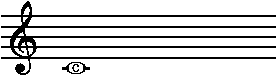
\includegraphics{notes/1c}
\end{center}

a half of a note ringing at d4:

\begin{Verbatim}[frame=single]
      staff foo {
        n 2, d4;
      }
\end{Verbatim}

\begin{center}
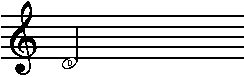
\includegraphics{notes/2d}
\end{center}

and a quarter of a note ringing at e4:
\begin{Verbatim}[frame=single]
      staff foo {
        n 4, e4;
      }
\end{Verbatim}

\begin{center}
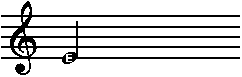
\includegraphics{notes/4e}
\end{center}

\np One can derive the length of the note from the denominator of these notes:
\verb+1/1 1/2 1/4+

\subparagraph{dyad}
The parameter \texttb{<note>} may be entered for a number of times:

\begin{Verbatim}[frame=single]
      staff foo {
        n 4, c4 e4 g4;
      }
\end{Verbatim}

\begin{center}
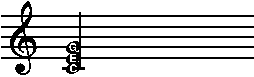
\includegraphics{notes/dyad_ceg}
\end{center}

\np The example above plays the C major chord at root position as whole note. (Integer overflow is not
protected; you might hear undesirable sounds.)

\np Dotted notes are implemented which reduces the duration of the playing of
that note. To use dots, you must to use a period. An example below is a 1/4 dotted note:
\begin{Verbatim}[frame=single]
      staff foo {
        n 4., c4;
        n 4..,d4;
      }
\end{Verbatim}

\begin{center}
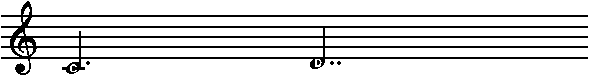
\includegraphics{notes/cpdpp}
\end{center}

\np There is no limit on how many dots you can enter; what's stopping you
is the limit to what the human ears can recognized.

\np The key from A-G is supported, and the octave it takes must be an integer
from 0 to 9.

\np To use accidentals, append \verb+#+ to the first letter of the note to raise the note a semitone and to lower the
note a semitone, append \verb+b+ to the first letter of the note:
\begin{Verbatim}[frame=single]
      staff foo {
        n 1, c#4;
        n 2, db4;
      }
\end{Verbatim}

\begin{center}
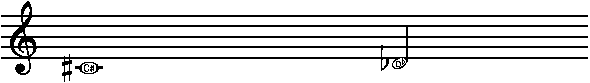
\includegraphics{notes/csdf}
\end{center}

\np Unlike the parameter \texttb{<length>}, arithmetic operation is illegal
to perform on a \texttb{<note>}. so \texttb{<note>+<note>} is prohibited.

\np To play a chord or a dyad, like \texttb{c4 e4 g4}, one just needs to write as it is:

\begin{Verbatim}[frame=single]
      n 4, c4 e4 g4;
\end{Verbatim}

\textbf{NOTE} If all these notes is played as staccato, append,
\texttb{.}, to them, so, it becomes, \texttb{c4. e4. g4.}

\paragraph{\texttb{<length>}} For argument, \texttb{<length>}, it may be in the form of integer or floating point number:
\label{nlength}

\begin{Verbatim}[frame=single]
      n 4.0, <note>;
      n 4, <note>;
\end{Verbatim}

\np To simulate a tie, use \verb-+-

\begin{Verbatim}[frame=single]
      n 4+4, 440; /* is equivalent to: */
      n 2, 440; 
\end{Verbatim}

\np How the former is equivalent to \texttb{n 2, 440;} might
not make sense as, $4+4$ is mathematically equal to 8. Instead
of treating this as an addition operation which sums up two
operands (which is confusing), consider to pronouce it as
\textit{four-tie-four} instead of \textit{four-plus-four}.
 
\textbf{NOTE} Other arithmetic operations are prohibited.

\np The paramater, \textgray{<length>}, will take any real positive integer (as long as it's in the range of int),
so a length of \verb+3+ will work (equivalent to 1/3 of a note), \verb+5+ will work (equivalent to 1/5
of a note) and others.

\np To play a 1/8 note triplet, one may need to do some math:

\begin{align}
	\shortintertext{Multiply 1/8 with 2:}
	\frac{1}{8}2 = \frac{2}{8} \Rightarrow \frac{1}{4} \\
	\shortintertext{divide the answer with 3 (3 for triplet):}
	\frac{1}{4(3)} = \frac{1}{12}
\end{align}

and use the denominator, \verb+12+, as the value of the length:
\begin{Verbatim}[frame=single]
      staff foo {
        n 12, c4;
        n 12, d4;
        n 12, e4;
      }
\end{Verbatim}

\begin{center}
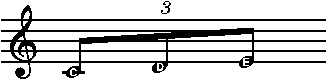
\includegraphics{notes/4triplet_cde}
\end{center}

This process can be repeates for 1/8 note quadruplet, but instead of dividing
with 3 in step (2), it's divided with 4 (4 for quadruplet) and so on.


\subsubsection{\textgray{r}}

\np The \verb+r+ keyword signifies the beginning of a musical rest. It must be
declared inside the \textit{staff block}. It takes one parameter; the
length of the rest:

\begin{Verbatim}[frame=single]
      r <length>;
\end{Verbatim}

\np The syntax of \texttb{<length>} is similar to the definition in 
\autoref{nlength}.

\subsubsection{Extensions}

\subsection{\textgray{track}}
\np A declaration of variable of type,
\verb+track+, must be immdediately followed by its identifier, followed by
an assignment to one of synthesizers taking a type, \verb+staff+. 
\begin{Verbatim}[frame=single]
       track foo = synth.psg(pol);
\end{Verbatim}

or other variable of type ,\verb+track+.
\begin{Verbatim}[frame=single]
      track foo = synth.psg(pol);
      track bar = foo;
\end{Verbatim}

\np To append these supported types, a comma must be added, followed by an rvalue:
\begin{Verbatim}[frame=single]
      track foo = synth.psg(bar), synth.psg(bar);
\end{Verbatim}


\subsubsection{Extensions}

\np The length of the rest is semantically similar to one of that length
of the note. Refer to the \verb+n+ keyword.

\subsection{Formatting}
\label{formatting}
\np To preserve the readability of the text, it is a recommended practice to add a comment for every
beginning measure, regardless of the time signature. Below is a 4/4 time signature:
\begin{Verbatim}[frame=single]
      staff foo {
        // Measure 1
        n 1, c4;
  
        // Measure 2
        n 4, d4;
        n 4, e4;
        n 4, f4;
        n 4, g4;
  
        // Measure 3
        n 2, a4;
        n 2, b4;
      }
\end{Verbatim}



\section{Staff block}
\paragraph{Syntax}
\begin{verbatim}
       <staff_blk> :         "staff" "{" <staff_blk_stmts> "}"
\end{verbatim}
\paragraph{Semantics}

\subparagraph{Pre-defined staff block variables \texttb{<staff\_blk\_var>}}
\begin{verbatim}
       <staff_blk_var> :     "octave"
                             "semitone"
                             "bpm"
\end{verbatim}

\paragraph{Constraints}

\subsection{Statements \texttb{<staff\_blk\_stmts>}}
\paragraph{Syntax}
\begin{verbatim}
       <staff_blk_stmts> :   <n_stmt> ";"
                             <r_stmt> ";
\end{verbatim}

\subsubsection{\textgray{n} \texttb{<n\_stmt>}}
\paragraph{Syntax}
\begin{verbatim}
       <n_stmt> :            <explicit_n>
                             <implicit_n>
 
       <explicit_n> :        "n" <length> "," <note>

       <implicit_n> :        <note> <length>

       <length> :            <numeric> [\.]*
                             <length> "+" <length>
\end{verbatim}

\paragraph{Semantics}
\paragraph{Constraints}

\subsubsection{\textgray{r} \texttb{<r\_stmt>}}
\begin{verbatim}
       <r_stmt> :            <explicit_r>
                             <implicit_r>

       <explicit_r> :        "r" <length>

       <implicit_r> :        <length>

       <length> :            <numeric> [\.]*
                             <length> "+" <length>
\end{verbatim}

\subsubsection{Assignment}



\section{Main block}
\paragraph{Syntax}


\paragraph{Semantics}
\paragraph{Constraints}



\section{Synths}
(A complete list of synths supported by dats can be listed by running \texttt{dats -{}-list-synths})

\np In this document, a synth takes a staff, (optionally, with arguments), and returns a pcm16.

\np Usually, a composer would like to spice things up, add some punch or tweak some
parameters of the synth, in this case, values or strings, may be passed to the options provided
by the synth. These are always enclosed in a bracket:

\begin{Verbatim}[frame=single]
      synth.synth_name(staff)[synth_option1=123];
\end{Verbatim}

Sucession of options can be done by appending a comma followed by an another option:

\begin{Verbatim}[frame=single]
      synth.synth_name(staff)[
          synth_option1=123,
          synth_option2=123,
          synth_option3="test"];
\end{Verbatim}

\np A list of options provided by a synth can be found by running,
\texttt{dats -{}-list-options synth\char`_name}. (not yet implemented)



\section{Filters}

In this document, a filter takes a track, (optionally, with arguments), and returns a track.

\section{EBNF}
%\section*{Afterword}
\renewcommand{\section}{\clearpage\setcounter{numpar}{0}\stdsection}

\end{document}
